\section{Matched optimization study}\label{sec:optimization}
The preceding sections establish that the gradients are accurate for the
model they differentiate. This section tests whether they shorten the time
needed to reach a common validated ripple target. The protocol and all of
its amendments were fixed in the
\href{https://github.com/rjwalters/geode-fem/issues/1185}{preregistration}
before any main-run outcome was observed. One later deviation, in how the
final refinement was run, was adopted after the main runs had finished and
is described with the refinement in Section~\ref{sec:exp2-refinement}; it
changes no selection rule, check or target.

\subsection{Protocol}
\paragraph{Methods.}
Five methods form an optimizer-by-resolution comparison plus one
surrogate (Table~\ref{tab:methods}). A and E are safeguarded SLSQP
\citep{kraft1988} using the field adjoints of Section~\ref{sec:gradients};
B and D are COBYQA \citep{ragonneau2022} with $2n+1$ interpolation points
and unit-box trust radii $0.1$ to $10^{-6}$, where $n$ is the number of free
parameters. Both run through SciPy 1.18.1 \citep{virtanen2020scipy}. C is
an empirical cubic radial-basis trust-region surrogate fitted to L1
evaluations. A/B and E/D vary the optimizer at fixed training resolution,
and A/E and B/D vary resolution at fixed optimizer. The optimizer contrast
includes differences in search strategy, so it does not isolate gradient
access as the only causal difference. Training uses order-45 coupling torque
on 20 angles at current fractions $0$, $\tfrac12$ and $1$ of the fixed peak
current $9.6777\,\mathrm{A}$. L0 and L1 differ only in spatial resolution,
and neither is fitted or corrected against validation. Time to a fixed
target, with unattained targets kept as censored, follows the data- and performance-profile
practice for benchmarking optimization solvers \citep{more2009benchmarking,dolan2002benchmarking}.
The preregistration also named a fixed group-1 current-density rule as a
labelled control. It was not run in this study, which uses the fixed
physical current throughout; Section~\ref{sec:gradients} reports that
rule's effect on sensitivities.

\begin{table}[H]\centering\small
\caption{Methods. D and E solve the coarse nonlinear field equations; they
are neither fitted magnetic circuits nor reduced-basis models.}
\label{tab:methods}
\begin{tabular}{lll}\toprule
Method & Optimizer or search model & Training mesh\\\midrule
A & Safeguarded SLSQP, field adjoints & L1\\
B & COBYQA, forward evaluations & L1\\
C & Empirical cubic-RBF trust region & L1\\
D & COBYQA, forward evaluations & L0\\
E & Safeguarded SLSQP, field adjoints & L0\\\bottomrule
\end{tabular}
\end{table}

\paragraph{Design spaces and constraints.}
Space A has eight free geometric lengths: MAG, MH, MW, SW1--SW4 and Sr1
(Appendix~\ref{sec:parameters}), that is, the rotor iron depth, magnet
height and width, four stator tooth and slot dimensions, and the slot-bottom
fillet radius. Space B adds ten grouped offsets acting on 55 surface control
points. Stack length, radial scale, stator outer diameter and operating
angle are fixed, so the saved Opt120 design lies outside both spaces. The
two spaces also use different discrete mesh-motion maps, so their contrast
does not isolate the ten added offsets.
Each training model $r\in\{\mathrm{L0},\mathrm{L1}\}$ minimizes
$F_r=\sum_c\sigma_{r,c}^2$ over the three training currents, subject to
$\mu_{r,1}\geq1.0025\,\mu_{r,1}(\theta_0)$ for its own full-current mean and to
normalized construction margins $c_i-0.05\geq0$. Unbuildable or
mesh-infeasible candidates are refused: SLSQP restores toward the last
admissible point and restarts, COBYQA receives a NaN barrier, and C skips
the point. A moved mesh with an inverted triangle or a minimum angle below
$5^\circ$ is repaired by up to four charged remeshing attempts. Because
refinement cannot remove a limiting geometric corner, the $5^\circ$ policy
also acts as an implicit geometric constraint. Space B's slot-opening
channel wall is not guarded and can become very thin at extreme offsets;
that risk is handled by repair and refusal, not by a wall-thickness
constraint.

\paragraph{Common validation and credit.}
Every method is judged on the same order-93, L2, 20-angle validation model.
Its initial-design anchor is $F_0=9.6034\times10^{-3}\,(\Nm)^2$ with
full-current mean $\mu_0=1.44084\,\Nm$. The targets are $T_{50}=0.5F_0$,
$T_{90}=0.1F_0$ and $T_{99}=0.01F_0$. A validated design attains a target
only if
\begin{equation}
 F_{\mathrm{val}}+\delta F\leq T,\qquad
 \delta F=\max\{0.10F_{\mathrm{val}},\,2.5\times10^{-7}\,(\Nm)^2\},
\end{equation}
its validated full-current mean is at least $1.0025\,\mu_0$, its
construction margins and mesh checks pass, and its validation completes
within budget. The allowance $\delta F$ is an empirical margin, not a bound
on continuum error. Optimizer success flags confer no credit. Changed
incumbents are validated as they appear, after the initial interpolation
set for B, C and D.

\paragraph{Budget and timing.}
Cost is wall time, in units of the median cold validation forward measured
on the same host at the same concurrency. Each run receives 120 units,
with a 60-unit checkpoint that counts only validations completed by then.
The charge covers evaluator start-up, geometry checks, mesh motion and
repair, training solves, adjoints, optimizer overhead, surrogate fitting
and validation; nothing is subtracted as overhead. L0 receives no discount.

\paragraph{Starts and execution.}
Each space uses $\theta_0$ and four Latin-hypercube starts (seeds 1--4),
with the scalar coordinates matched across spaces. A start was eligible
only if it was buildable and admissible, and its moved reference mesh met
the mesh policy without repair, in both spaces at L0 and L1. The starts
therefore favor moderate deformations and are not uniform samples of the
design box. All starts were frozen before any main outcome. Every method
runs from every start twice, giving 100 runs. Within a start, repeat 1
rotates the method order and repeat 2 reverses it.

The session ran on one AWS c7a.4xlarge host (x86-64; NumPy 2.5.4 and
SciPy 1.18.1 with OpenBLAS) with 15 concurrent single-threaded processes.
Before calibration, the host recomputed the initial-design validation
waveforms in both spaces. $F_0$ agreed with the canonical anchor to
$2.4\times10^{-13}$ relative, within the preregistered $10^{-9}$ tolerance,
and the two spaces agreed bit for bit. The calibrated unit was
$70.94\,\mathrm{s}$, the median of 45 concurrent cold validations. All 100
runs completed in one session with no recovery, deferral or contamination:
the one-minute load average peaked at 21.1, below the contamination
threshold of $1.5N=22.5$. The in-run cost totals 109~CPU-hours. Of the
100 runs, 38 stopped on reaching $T_{99}$, 46 on optimizer convergence and
13 at the budget. The other three are SLSQP runs (A) in space A whose
solver stopped without converging: both repeats from LHS~2, after about 43
units, and repeat~1 from LHS~3, after 119 units.

\subsection{Results}
\paragraph{Repeats.}
The two repeats of each run follow the same optimization path. In all 50
pairs, the sequences of validated objectives agree exactly up to the
shorter run's length, and they differ in length only when the budget or a
solver stop cuts one repeat earlier. The repeats therefore measure timing
noise, not independent outcomes, and the comparison is a paired case study
over five starts. Over the 111 target crossings attained in both repeats,
the time differs by a median of 2.1\% and at most 12.4\% relative to
repeat~1. Repeat-1 times are reported below.

\paragraph{Attained quality.}
Figure~\ref{fig:exp2-quality} shows the best credited value of
$(F+\delta F)/F_0$ for every start, method and space (repeat~1).
In space A, no run goes below $F/F_0=0.043$ and none reaches $T_{99}$.
The best designs of A, B, D and E all reach $0.043F_0$, and C's reaches
$0.049F_0$; in Fig.~\ref{fig:exp2-quality}, which includes the allowance,
the A, B, D and E level appears near $0.048$ (C's near $0.054$). All five lie within 0.17\% above the
full-current mean floor, so the mean constraint is active there: the level
shared by A, B, D and E is the constrained optimum they found in the
eight-parameter space,
not a property of any one method. In space A the start mattered more than
the method. From LHS~4, A and B stop near $0.09F_0$, D reaches $0.044F_0$,
and C and E never produce a credited validation, in either repeat. In
space B, each method's best design reaches $0.004$--$0.009F_0$, and every
method except C reaches $T_{99}$ from at least four of five starts.

\begin{figure}[t]\centering
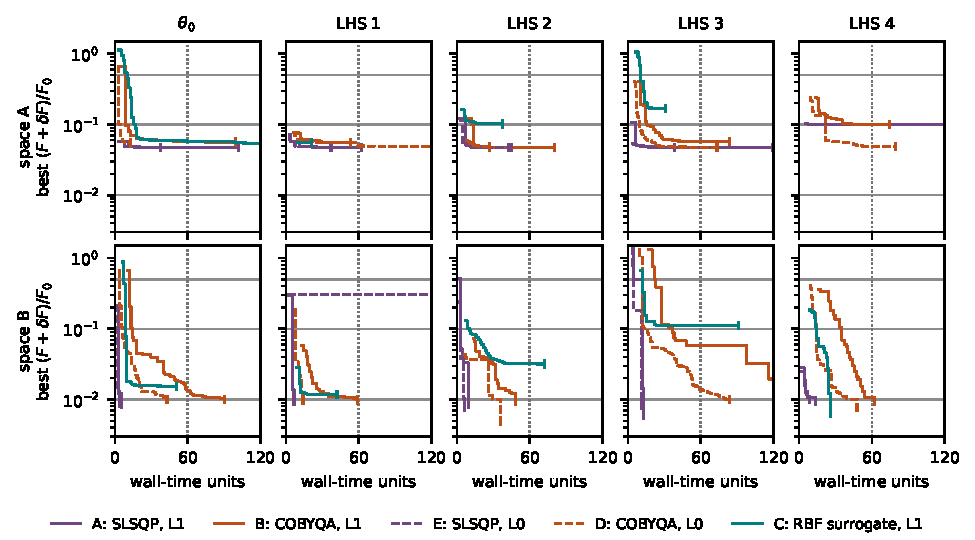
\includegraphics[width=\linewidth]{figures/exp2-quality.pdf}
\caption{Best credited $(F_{\mathrm{val}}+\delta F)/F_0$ versus charged wall
time, repeat~1, at common L2/order-93/20-angle validation. Grey lines mark
$T_{50}$, $T_{90}$ and $T_{99}$; the dotted line marks the 60-unit
checkpoint. Each curve ends at the run's actual stop (tick). A missing curve
means the run had no credited validation.}
\label{fig:exp2-quality}
\end{figure}

\paragraph{Time to target.}
Table~\ref{tab:exp2-time} and Figure~\ref{fig:exp2-time} give the charged
time to each target, per start. In repeat~1, only three crossings occur
after the 60-unit checkpoint, all at $T_{99}$ in space B: two by B and one
by D.

Table~\ref{tab:exp2-ratios} gives paired time ratios. A ratio is formed
only when both methods attain the target from that start; no finite ratio
is derived from a censored cell. Wherever both reach a target from the
same start, gradient-based SLSQP gets there sooner than COBYQA at the same
training resolution. At L1 (B/A), the geometric-mean ratio is 3.10--3.25 in
space A and 5.06--7.79 in space B. At L0 (D/E), it is 2.45--2.75 and
3.14--7.20.
All 45 finite optimizer-contrast pairs (by space, target and start) favor
SLSQP, with ratios from 1.46 to 21.5. The coarse mesh shortens the time by
a smaller factor: the geometric-mean E/A ratio is 0.62--0.79 and D/B is
0.45--0.56. Against D, the inexpensive derivative-free physical competitor,
A is faster by a geometric mean of 1.68--1.83 in space A and 2.25--4.32 in
space B. This contrast changes both factors; one of its 25 pairs is a near tie
(0.99, space-A LHS~2 at $T_{90}$: D is 0.75\% faster, within the timing
noise between repeats). We conjecture that part of the larger
space-B ratios comes from COBYQA's initial interpolation set, which costs
$2n+1=37$ training evaluations before its first model step there, against
17 in space A.

The speed of E has a reliability cost. E never produces a credited
validation from space-A LHS~4. From space-B LHS~1 it reaches $T_{50}$ but
then stalls at $0.28F_0$, missing $T_{90}$ and $T_{99}$. In four
start--target cells, D reaches a target that E misses. A, by contrast,
reaches every target that any method reaches, from every start. C attains
$T_{99}$ only once in space B and reaches $T_{90}$ from two of five
space-A starts.

\begin{figure}[t]\centering
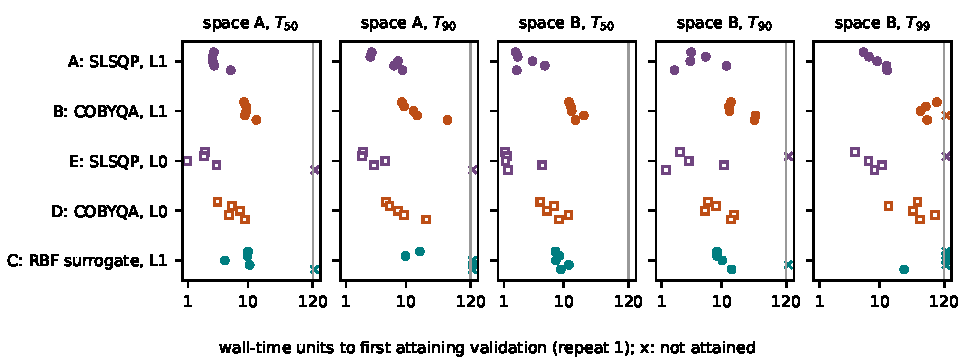
\includegraphics[width=\linewidth]{figures/exp2-time-to-target.pdf}
\caption{Charged wall time to the first attaining validation, repeat~1, one
marker per start, for every target attained by some run. Filled markers:
L1 training; open markers: L0 training; crosses: not attained within 120
units.}
\label{fig:exp2-time}
\end{figure}

\begin{table}[H]\centering\small
\caption{Charged wall-time units to the first attaining validation,
repeat~1. A dash means the target was not attained within 120 units.
$T_{99}$ was attained by no run in space A.}
\label{tab:exp2-time}\begin{tabular}{llrrrrr}\toprule
Space, target & Method & $\theta_0$ & LHS 1 & LHS 2 & LHS 3 & LHS 4\\\midrule
A, $T_{50}$ & A & 2.7 & 2.5 & 2.6 & 2.7 & 5.1\\
 & B & 8.5 & 9.3 & 9.3 & 8.9 & 13.7\\
 & E & 1.9 & 1.8 & 1.0 & 3.0 & ---\\
 & D & 3.1 & 5.3 & 7.3 & 4.8 & 8.8\\
 & C & 10.0 & 9.8 & 4.1 & 10.6 & ---\\
\addlinespace
A, $T_{90}$ & A & 2.7 & 2.5 & 7.4 & 6.4 & 8.8\\
 & B & 8.5 & 9.3 & 13.3 & 15.4 & 49.3\\
 & E & 1.9 & 1.8 & 4.5 & 3.0 & ---\\
 & D & 4.6 & 5.3 & 7.3 & 9.4 & 21.9\\
 & C & 16.9 & 9.8 & --- & --- & ---\\
\addlinespace
B, $T_{50}$ & A & 1.6 & 1.7 & 3.0 & 4.8 & 1.6\\
 & B & 12.2 & 13.1 & 13.5 & 21.5 & 15.7\\
 & E & 1.0 & 1.1 & 1.1 & 4.4 & 1.2\\
 & D & 4.1 & 6.9 & 5.2 & 11.9 & 8.4\\
 & C & 7.3 & 8.4 & 7.3 & 12.1 & 8.9\\
\addlinespace
B, $T_{90}$ & A & 3.1 & 5.4 & 3.0 & 12.0 & 1.6\\
 & B & 14.4 & 13.1 & 13.5 & 36.6 & 35.3\\
 & E & 2.0 & --- & 2.8 & 10.9 & 1.2\\
 & D & 5.9 & 8.1 & 5.2 & 15.9 & 14.3\\
 & C & 8.4 & 8.4 & 10.3 & --- & 14.6\\
\addlinespace
B, $T_{99}$ & A & 5.4 & 6.6 & 9.1 & 13.1 & 13.4\\
 & B & 90.4 & 59.1 & 48.6 & --- & 62.3\\
 & E & 3.9 & --- & 6.5 & 10.9 & 8.3\\
 & D & 43.0 & 14.1 & 36.0 & 83.3 & 47.8\\
 & C & --- & --- & --- & --- & 25.9\\
\bottomrule\end{tabular}

\end{table}

\begin{table}[H]\centering\small
\caption{Paired per-start time ratios (repeat~1). B/A and D/E vary the
optimizer at fixed resolution; E/A and D/B vary the resolution; D/A
compares A with the coarse derivative-free competitor. Ratios above one
favor the denominator. Geometric means use the finite pairs only, so the
D/E and E/A means omit the starts where E failed to attain the target.}
\label{tab:exp2-ratios}\begin{tabular}{llrrl}\toprule
Space, target & Ratio & Finite pairs & Geometric mean & Per-start ratios\\\midrule
A, $T_{50}$ & B/A & 5 & 3.25 & 3.18, 3.66, 3.63, 3.25, 2.66\\
 & D/E & 4 & 2.75 & 1.60, 2.90, 7.68, 1.61, ---\\
 & E/A & 4 & 0.68 & 0.72, 0.72, 0.37, 1.09, ---\\
 & D/B & 5 & 0.56 & 0.36, 0.57, 0.78, 0.54, 0.64\\
 & D/A & 5 & 1.83 & 1.15, 2.09, 2.85, 1.75, 1.71\\
\addlinespace
A, $T_{90}$ & B/A & 5 & 3.10 & 3.18, 3.66, 1.80, 2.43, 5.61\\
 & D/E & 4 & 2.45 & 2.41, 2.90, 1.61, 3.17, ---\\
 & E/A & 4 & 0.62 & 0.72, 0.72, 0.61, 0.47, ---\\
 & D/B & 5 & 0.54 & 0.54, 0.57, 0.55, 0.61, 0.44\\
 & D/A & 5 & 1.68 & 1.72, 2.09, 0.99, 1.48, 2.49\\
\addlinespace
B, $T_{50}$ & B/A & 5 & 6.49 & 7.76, 7.70, 4.51, 4.46, 9.59\\
 & D/E & 5 & 4.69 & 3.90, 6.14, 4.93, 2.72, 7.09\\
 & E/A & 5 & 0.63 & 0.66, 0.66, 0.35, 0.91, 0.72\\
 & D/B & 5 & 0.46 & 0.33, 0.52, 0.39, 0.56, 0.53\\
 & D/A & 5 & 2.97 & 2.58, 4.04, 1.75, 2.48, 5.09\\
\addlinespace
B, $T_{90}$ & B/A & 5 & 5.06 & 4.64, 2.41, 4.51, 3.05, 21.54\\
 & D/E & 4 & 3.14 & 2.94, ---, 1.86, 1.46, 12.17\\
 & E/A & 4 & 0.79 & 0.65, ---, 0.94, 0.91, 0.72\\
 & D/B & 5 & 0.45 & 0.41, 0.62, 0.39, 0.44, 0.41\\
 & D/A & 5 & 2.25 & 1.91, 1.50, 1.75, 1.33, 8.74\\
\addlinespace
B, $T_{99}$ & B/A & 4 & 7.79 & 16.65, 8.92, 5.33, ---, 4.65\\
 & D/E & 4 & 7.20 & 11.05, ---, 5.50, 7.65, 5.79\\
 & E/A & 4 & 0.72 & 0.72, ---, 0.72, 0.83, 0.61\\
 & D/B & 4 & 0.50 & 0.48, 0.24, 0.74, ---, 0.77\\
 & D/A & 5 & 4.32 & 7.91, 2.12, 3.94, 6.36, 3.56\\
\bottomrule\end{tabular}

\end{table}

\paragraph{Final refinement.}\label{sec:exp2-refinement}
The preregistered selection takes, for each method and space, the
lowest-$F_{\mathrm{val}}$ feasible design over both repeats, and the
earliest repeat-1 crossing of each attained target. With $\theta_0$ in
each space and identical designs merged, this gives 33 designs. Each
received the six registered checks: the primary L2 validation, L3, a
40-angle grid, Newton tolerance $10^{-12}$, an independently solved grid
shifted by $0.5^\circ$, and held-out currents $0.25$ and $0.75$. The 15
designs with zero stator offsets also received the conforming outer-band
Arkkio check on fresh meshes. All 213 checks completed
(Table~\ref{tab:exp2-refinement}). These checks qualify the selected
designs only; they do not certify each of the study's 111 repeat-1
target crossings.

The registered pipeline begins by capturing the closed study on its
original host. After that host had been restarted, the capture tool
repeatedly refused on host-boot attestation details unrelated to the
data. The refinement instead used a copy of the study outputs whose
integrity is established by a SHA-256 inventory of every output file, taken
when the session finished, before the host was restarted, and
independently timestamped. It ran on a different host (Apple M3 Ultra,
macOS arm64). For the 16 selected designs validated on the moved reference
mesh, the primary check reproduces the study's $F_{\mathrm{val}}$ to below
$2.2\times10^{-12}$ relative. The other 15 candidates needed a fresh mesh,
which Gmsh triangulates differently on the two platforms; their $F$
differs by at most $1.7\times10^{-3}$ relative. The remaining two designs
are $\theta_0$ in each space, which reproduces $F_0$. The fresh-mesh
differences measure the sensitivity of $F$ to remeshing and are far below
the 10\% allowance $\delta F$.

Spatial refinement is the largest change. Over all 33 designs, L3 moves
$F$ by $-4.0\%$ to $+6.3\%$. Over the 25 target crossings alone, the range
is $-4.0\%$ to $+1.1\%$. The largest increase belongs to the overall best
design, D's in space B, whose $F$ rises from $0.0044F_0$ to $0.0047F_0$.
Angular and nonlinear effects are small: the 40-angle and shifted grids
change $F$ by at most $0.11\%$, and the tighter Newton tolerance by less
than $1.1\times10^{-5}$ relative. The conforming estimator gives $1.1\%$ to
$4.4\%$ more ripple than the order-93 coupling on the space-A designs, and
$2.0$--$2.1\%$ more at $\theta_0$. All 25 target crossings still satisfy
their target, allowance included, at L3; the smallest remaining margin is
1.2\% of the target. Every candidate also satisfies the full-current mean
floor in the primary, L3, 40-angle, tight and shifted checks, the closest
by 0.012\%. The refinement therefore confirms the selected crossings and
leaves the time-to-target comparison unchanged.

The held-out currents test the ripple reduction outside the three training
currents. We compare each design's objective at currents $0.25$ and $0.75$,
relative to $\theta_0$'s at the same currents, with its relative objective
at the training currents. Across the candidates, the held-out ratio is 0.65
to 1.73 times the training-current ratio; values above one mean a smaller
reduction at the held-out currents. For the five best space-A designs it
is 1.07--1.09. In space B, four of the five best designs keep less of
their reduction: their remaining objective fraction at the held-out currents
is 1.23--1.73 times that at the training currents, while for B's best
design it is 0.89. D's best design has $0.0044F_0$ at the training currents but
$0.0076$ of $\theta_0$'s value at the held-out currents. Part of the extra
reduction from space B's added freedom is therefore specific to the three
training currents.

\begin{table}[H]\centering\scriptsize
\caption{Final checks of the selected designs. ``best'' marks a method's
representative; ``A $T_{90}$'' marks the earliest repeat-1 crossing of that
target by that method. The L2 column is the primary check on the
refinement host. L3 and conforming changes are in percent; the 40-angle,
tight and shifted changes are relative, in units of $10^{-4}$. ``held-out'' is the objective at currents $0.25$ and
$0.75$ relative to $\theta_0$'s at the same currents. A dash means the
conforming check does not apply because stator offsets are nonzero.}
\label{tab:exp2-refinement}\begin{tabular}{lrrrrrrr}\toprule
Design & $F_{\mathrm{L2}}/F_0$ & L3 & g40 & tight & shifted & conf. & held-out\\
 & & (\%) & ($10^{-4}$) & ($10^{-4}$) & ($10^{-4}$) & (\%) & \\\midrule
\multicolumn{8}{l}{\emph{Space A}}\\
$\theta_0$ & 1.0000 & $-1.3$ & $0.0$ & $0.0$ & $+0.1$ & $+2.1$ & 1.0000\\
best A & 0.0432 & $-0.4$ & $0.0$ & $0.0$ & $+0.1$ & $+4.4$ & 0.0472\\
best B & 0.0432 & $-0.5$ & $0.0$ & $0.0$ & $0.0$ & $+4.4$ & 0.0472\\
best C & 0.0489 & $-0.7$ & $+0.2$ & $0.0$ & $+0.5$ & $+4.1$ & 0.0524\\
best D & 0.0432 & $-0.5$ & $0.0$ & $0.0$ & $0.0$ & $+4.4$ & 0.0472\\
best E & 0.0434 & $-0.6$ & $+0.4$ & $0.0$ & $+0.9$ & $+4.4$ & 0.0473\\
A $T_{50}$, A $T_{90}$ & 0.0653 & $-2.9$ & $+0.7$ & $0.0$ & $+1.5$ & $+1.1$ & 0.0686\\
B $T_{50}$, B $T_{90}$ & 0.0881 & $-2.3$ & $+1.3$ & $0.0$ & $+2.6$ & $+3.2$ & 0.0866\\
C $T_{50}$ & 0.1472 & $-4.0$ & $+0.6$ & $0.0$ & $+1.3$ & $+3.3$ & 0.1508\\
C $T_{90}$ & 0.0507 & $-0.9$ & $+0.2$ & $0.0$ & $+0.5$ & $+4.0$ & 0.0543\\
D $T_{50}$ & 0.0920 & $-2.2$ & $+1.5$ & $0.0$ & $+3.0$ & $+3.3$ & 0.0899\\
D $T_{90}$ & 0.0594 & $-2.3$ & $+1.3$ & $0.0$ & $+2.6$ & $+1.6$ & 0.0609\\
E $T_{50}$ & 0.1105 & $-2.0$ & $+0.6$ & $0.0$ & $+1.1$ & $+1.2$ & 0.1104\\
E $T_{90}$ & 0.0660 & $-2.9$ & $+0.7$ & $0.0$ & $+1.5$ & $+1.1$ & 0.0694\\
\multicolumn{8}{l}{\emph{Space B}}\\
$\theta_0$ & 1.0000 & $-1.3$ & $0.0$ & $0.0$ & $+0.1$ & $+2.0$ & 1.0000\\
best A & 0.0053 & $+2.6$ & $+0.4$ & $+0.1$ & $+0.5$ & --- & 0.0066\\
best B, B $T_{99}$ & 0.0085 & $-3.0$ & $-0.4$ & $0.0$ & $-1.2$ & --- & 0.0076\\
best C, C $T_{99}$ & 0.0057 & $-3.7$ & $+2.5$ & $0.0$ & $+5.0$ & --- & 0.0074\\
best D & 0.0044 & $+6.3$ & $+2.6$ & $+0.1$ & $+4.9$ & --- & 0.0076\\
best E & 0.0071 & $+2.6$ & $-1.5$ & $0.0$ & $-3.1$ & --- & 0.0087\\
A $T_{50}$ & 0.1874 & $+0.9$ & $-0.3$ & $0.0$ & $-0.6$ & --- & 0.1538\\
A $T_{90}$ & 0.0255 & $+1.1$ & $-0.1$ & $0.0$ & $-0.2$ & --- & 0.0248\\
A $T_{99}$ & 0.0077 & $+0.4$ & $-0.1$ & $0.0$ & $-0.3$ & --- & 0.0096\\
B $T_{50}$ & 0.1854 & $-1.5$ & $-0.1$ & $0.0$ & $-0.3$ & --- & 0.1907\\
B $T_{90}$ & 0.0523 & $-0.4$ & $-0.2$ & $0.0$ & $-0.4$ & --- & 0.0505\\
C $T_{50}$ & 0.3958 & $-1.4$ & $-0.1$ & $0.0$ & $-0.1$ & --- & 0.3692\\
C $T_{90}$ & 0.0259 & $+0.7$ & $0.0$ & $0.0$ & $0.0$ & --- & 0.0247\\
D $T_{50}$ & 0.1925 & $-1.5$ & $-0.1$ & $0.0$ & $-0.3$ & --- & 0.1971\\
D $T_{90}$ & 0.0393 & $-0.7$ & $+0.6$ & $0.0$ & $+1.2$ & --- & 0.0392\\
D $T_{99}$ & 0.0089 & $+0.4$ & $-0.5$ & $0.0$ & $-1.0$ & --- & 0.0137\\
E $T_{50}$ & 0.1961 & $+0.8$ & $0.0$ & $0.0$ & $0.0$ & --- & 0.1567\\
E $T_{90}$ & 0.0223 & $-2.8$ & $-5.3$ & $0.0$ & $-10.6$ & --- & 0.0144\\
E $T_{99}$ & 0.0081 & $+0.7$ & $+0.2$ & $0.0$ & $+0.4$ & --- & 0.0112\\
\bottomrule\end{tabular}

\end{table}
